\documentclass[10pt,a4paper]{article}
\usepackage[utf8]{inputenc}
\usepackage[T1]{fontenc}
\usepackage{lmodern}
\usepackage[english]{babel}
\usepackage[margin=2.0cm]{geometry}
\usepackage{amsmath,amssymb,mathtools,bm}
\usepackage{booktabs,array,tabularx}
\newcolumntype{L}[1]{>{\raggedright\arraybackslash}p{#1}}
\usepackage{graphicx}
\usepackage{float}
\usepackage[font=small]{caption}
\usepackage{xcolor}
\usepackage{tikz}
\usetikzlibrary{arrows.meta,positioning,calc}
\usepackage[hidelinks]{hyperref}
\usepackage{url}
\makeatletter\g@addto@macro{\UrlBreaks}{\do\_\do/}\makeatother
\numberwithin{equation}{section}
\setlength{\emergencystretch}{3em}
\newcommand{\note}[1]{\begin{center}\fcolorbox{red!70!black}{red!5}{\parbox{0.94\linewidth}{\small\textbf{Note.} #1}}\end{center}}
\newcommand{\overlapShare}{54}
\newcommand{\gridOffset}{10^{-12}}
\newcommand{\olAR}{42.4}
\newcommand{\clpAR}{96.0}
\newcommand{\cliAR}{20.1}
\newcommand{\olAL}{42.4}
\newcommand{\clpAL}{96.0}
\newcommand{\cliAL}{20.1}
\newcommand{\olAF}{53.1}
\newcommand{\clpAF}{95.8}
\newcommand{\cliAF}{25.6}
\newcommand{\olPR}{13.3}
\newcommand{\clpPR}{95.7}
\newcommand{\cliPR}{50.1}
\newcommand{\olPL}{13.3}
\newcommand{\clpPL}{95.7}
\newcommand{\cliPL}{50.0}
\newcommand{\olPF}{$-$3.2}
\newcommand{\clpPF}{95.7}
\newcommand{\cliPF}{46.4}
\newcommand{\sigmaHP}{17837}
\newcommand{\sigmaRP}{18782}
\newcommand{\sigmaFP}{20275}
\newcommand{\sigmaStdP}{7.4\,\%}
\newcommand{\TcHP}{0.407}
\newcommand{\gKtP}{1.05}
\newcommand{\gKtFP}{0.96}
\newcommand{\preslP}{23}
\newcommand{\TcFreeP}{0.385}
\newcommand{\TcFreeFP}{0.439}
\newcommand{\TsTP}{1.14}
\newcommand{\fitHP}{78.1 / 78.1 / 75.7}
\newcommand{\fitRP}{77.9 / 76.9 / 79.7}
\newcommand{\fitFP}{76.7 / 79.5 / 74.7}
\newcommand{\lowHP}{82.8}
\newcommand{\lowRP}{82.5}
\newcommand{\lowFP}{77.0}
\newcommand{\ArangeP}{1--3282}
\newcommand{\sigmaHA}{1571}
\newcommand{\sigmaRA}{1571}
\newcommand{\sigmaFA}{1560}
\newcommand{\sigmaStdA}{1.9\,\%}
\newcommand{\TcHA}{0.232}
\newcommand{\gKtA}{0.90}
\newcommand{\gKtFA}{0.90}
\newcommand{\preslA}{147}
\newcommand{\TcFreeA}{0.204}
\newcommand{\TcFreeFA}{0.144}
\newcommand{\TsTA}{7.93}
\newcommand{\fitHA}{75.3}
\newcommand{\fitRA}{75.3}
\newcommand{\fitFA}{72.6}
\newcommand{\lowHA}{89.8}
\newcommand{\lowRA}{89.8}
\newcommand{\lowFA}{79.2}
\newcommand{\ArangeA}{2--443}
\newcommand{\fMassI}{56.1}
\newcommand{\fMassII}{98.3}
\newcommand{\zMassI}{0.021}
\newcommand{\zMassII}{0.030}
\newcommand{\aMassI}{$-$0.548}
\newcommand{\aMassII}{0.591}
\newcommand{\zForkA}{0.028}
\newcommand{\alphaA}{0.607}
\newcommand{\kLA}{\ensuremath{5.47\times10^{4}}}
\newcommand{\Kt}{0.258}
\newcommand{\icmdMaxA}{12.2}
\newcommand{\akdErrA}{302}
\newcommand{\akdErrMeasA}{1297}
\newcommand{\akdImaxA}{77}
\newcommand{\akdImaxMeasA}{10.7}
\newcommand{\clFitMinA}{95.7}
\newcommand{\clFitMaxA}{99.5}
\newcommand{\iRatioMedA}{1.13}
\newcommand{\iRatioMinA}{1.03}
\newcommand{\iRatioMaxA}{1.19}
\newcommand{\icmdMaxP}{6.1}
\newcommand{\akdErrP}{3908}
\newcommand{\akdErrMeasP}{1316}
\newcommand{\akdImaxP}{5}
\newcommand{\akdImaxMeasP}{6.1}
\newcommand{\clFitMinP}{94.9}
\newcommand{\clFitMaxP}{99.3}
\newcommand{\iRatioMedP}{1.00}
\newcommand{\iRatioMinP}{0.80}
\newcommand{\iRatioMaxP}{1.13}
\newcommand{\quadResidual}{4 / 8 / 17 / 11}
\newcommand{\quadSignal}{0.8 / 1.4 / 4.1 / 2.7}


\tikzset{
  lab/.style={font=\scriptsize, inner sep=1.5pt},
  sig/.style={-{Latex[length=2mm]}, thick},
  blk/.style={draw, rounded corners, align=center, minimum height=0.9cm, fill=blue!4, font=\small},
  sum/.style={draw, circle, inner sep=1.2pt, font=\scriptsize},
}

\title{Fork modes and bearing friction of the LUCY mount:\\ Dahl model identified with an unweighted cost on uniformly sampled frequency responses}
\author{Generated by \texttt{build\_dahl\_resampled\_report.py}\\ \small\texttt{sim/gimbal\_multidof/report\_dahl\_resampled}}
\date{\today}
\begin{document}
\maketitle

\paragraph{Purpose.} The report \path{report_dahl_bearings} identifies the fork model with Dahl bearings by weighted least squares, with a weight $w_i=\sqrt{\Delta\ln f_i/0.01}$ on each measured point. This report removes the weight. The frequency responses are interpolated linearly between the measured points and sampled uniformly with the same number of points as each record, and the cost is $e^2=\sum(\Delta\mathrm{Re}^2+\Delta\mathrm{Im}^2)$. Model, constraints, data and verification are otherwise unchanged. The results are checked on the same three kinds of data:
\begin{itemize}
\item the \textbf{frequency responses} measured with WorkBench (fit band 1--150\,Hz), now also with fit values on the Bode magnitude and phase;
\item the \textbf{doublets} in \textbf{open loop}, driven by the measured motor current;
\item the same doublets in \textbf{closed loop}, driven by the measured position reference through the model of the AKD2G drive.
\end{itemize}

\paragraph{Main results.}
\begin{itemize}
\item \textbf{Adopted method: uniform in $\ln f$.} ``Uniform'' can mean uniform in $f$ or in $\ln f$, and both were run. The measured grids are already geometric, so the uniform $\ln f$ grid falls on the measured points (largest offset below $\gridOffset\,\%$). The interpolation then has no effect and the cost is the plain unweighted sum over the measured points. This grid is the one adopted here; the uniform $f$ grid is reported next to it.
\item \textbf{Effect on the estimate, uniform in $\ln f$.} The azimuth estimate is identical to the previous one, because its weight was a constant factor. In elevation only the 16-screw record changes weight, from $w^2\approx2$ to 1: $\sigma_0$ goes from \sigmaRP\ to \sigmaHP\,N\,m/rad, and the fit on the three records goes from \fitRP\,\% to \fitHP\,\%. Azimuth: $T_c=\TcHA$\,N\,m, $\sigma_0=\sigmaHA$\,N\,m/rad (std \sigmaStdA). Elevation: $T_c=\TcHP$\,N\,m, $\sigma_0=\sigmaHP$\,N\,m/rad (std \sigmaStdP).
\item \textbf{Effect of the uniform $f$ grid.} It moves the cost to high frequency: between 1 and 5\,Hz the main elevation record keeps 14 points out of 504 and the azimuth record 5 out of 170. The complex fit in 1--5\,Hz falls from \lowHP\ to \lowFP\,\% in elevation and from \lowHA\ to \lowFA\,\% in azimuth, and $g_{K_t}$ in elevation moves from \gKtP\ to \gKtFP. In azimuth the Bode magnitude and phase fits improve (Table~\ref{tab:bode}).
\item \textbf{Time domain.} With uniform $\ln f$ the doublets are the same as in the previous report. The median open-loop position fit during the moves is \olAL\,\% in azimuth and \olPL\,\% in elevation. In closed loop it is \clpAL\,\% and \clpPL\,\%. With uniform $f$ the open-loop fit changes in opposite directions (\olAF\,\% in azimuth, \olPF\,\% in elevation), and the closed-loop position fit stays within 0.3 points.
\end{itemize}

\note{The H7 configuration still contains placeholder data (inertias of the encoder and motor nodes, materials); the figures carry the label ``result from placeholder parameters''. The motor current of the doublets is the PLC channel \texttt{AXIS*\_AMPS}, taken as $2I_\mathrm{rms}$ as in \path{closedLoopModel}; that scale is not documented (Section~\ref{sec:limits}).}

\tableofcontents

%% ===================================================================================================
\section{Data}\label{sec:data}
\paragraph{Frequency responses.} The four WorkBench ``Plant'' responses of 28/10/2026, encoder velocity over motor current in (rad/s)/A$_\mathrm{rms}$:
\begin{itemize}
\item elevation: 1--600\,Hz on a 1\,\% grid, 30--150\,Hz on a 1\,\% grid, and 30--300\,Hz on a 2\,\% grid with 16 ring screws at 4\,A;
\item azimuth: 1--600\,Hz on a 3\,\% grid, 3.5\,A.
\end{itemize}
Only the points between 1 and 150\,Hz are fitted; Table~\ref{tab:sampling} gives their number. The exports also contain the controller and open-loop traces; the open loop is used to compute the motion of the bearings during the tests (Section~\ref{sec:df}).

\paragraph{Doublets.} \path{LucyIdentification/VClosedLoop/V2}, recorded on 20/10/2026 by the PLC at 2\,kHz: one axis per file, three moves $+A$, $-2A$, $+A$ at 10$^\circ$/s with rests of about 35\,s. Amplitudes used: 0.1, 0.5, 1, 3, 5 and 8$^\circ$ on each axis, i.e.\ 18 moves per axis. Channels: position reference and encoder position (millidegrees), and motor current \texttt{AXIS*\_AMPS} (\texttt{AXIS1} azimuth, \texttt{AXIS2} elevation). Each move is a window from 0.5\,s before the reference starts to 12\,s after it, or to the next move.

\paragraph{Drives.} \path{Parameters_azimuth.akd} and \path{Parameters_elevation.akd}, with gains and filters of the WorkBench exports of the same session (\path{V2/BodeMeasurement_*.csv}).

%% ===================================================================================================
\section{Model}\label{sec:model}
\subsection{Structure in modal form}
Each axis is the lumped model of \path{report_fork_modes}: elevation with the telescope rigid on the ring and two modal masses on the motor stator, azimuth with the load split into fork base and fork top. The bearings are removed from the stiffness:
\begin{equation}
\mathbf M\ddot{\mathbf x}+\mathbf C\dot{\mathbf x}+\mathbf K_0\mathbf x=\mathbf e\,\tau_m-\mathbf v\,T_b,\qquad \theta_\mathrm{enc}=\mathbf c^T\mathbf x,\qquad \delta=\mathbf v^T\mathbf x .\label{eq:struct}
\end{equation}
\begin{itemize}
\item $\tau_m$ is the motor torque. $\mathbf e$ applies it to the rotor and, in elevation, its reaction to the stator modal masses.
\item $\delta$ is the bearing deflection: hub minus stator structure in elevation, fork base minus ground in azimuth. $T_b$ is the friction torque that the bearings transmit.
\item The modes of $(\mathbf M,\mathbf K_0)$, $\mathbf K_0\bm\phi_k=\omega_k^2\mathbf M\bm\phi_k$ with $\bm\Phi^T\mathbf M\bm\Phi=\mathbf I$, now include the rigid rotation of the axis ($\omega_1\simeq0$). Each mode has its own viscous modal damping, so that $\mathbf C=\mathbf M\bm\Phi\,\mathrm{diag}(2\zeta_k\omega_k)\,\bm\Phi^T\mathbf M$.
\end{itemize}

\subsection{Dahl friction in the bearings}
The bearings are a Dahl element acting on $\delta$. Its internal state $z$ is the mean deflection of the contact asperities (the ``bristles''):
\begin{equation}
\frac{dz}{dt}=\dot\delta-\frac{\sigma_0\,|\dot\delta|}{T_c}\,z,\qquad T_b=\sigma_0 z .\label{eq:dahl}
\end{equation}
\begin{itemize}
\item \textbf{Pre-sliding.} For small motion, $|\sigma_0 z|\ll T_c$, the element is a spring of stiffness $\sigma_0$.
\item \textbf{Sliding.} For motion well beyond the pre-sliding scale $T_c/\sigma_0$, $T_b\to T_c\,\mathrm{sign}(\dot\delta)$: Coulomb friction.
\item The transition between the two regimes is smooth and hysteretic. The dissipation per cycle depends on the amplitude, not on the frequency.
\end{itemize}
The Dahl model is the LuGre model with static torque equal to the Coulomb torque ($T_s=T_c$) and no micro-damping or viscous term ($\sigma_1=\sigma_2=0$). LuGre with all six parameters was also identified; it fits the frequency responses only slightly better and its parameters are not identifiable (\path{report_dahl_bearings}).

\subsection{Frequency domain: describing function}\label{sec:df}
\paragraph{Describing function.} Under a sinusoidal deflection $\delta=A\sin\omega t$, the first harmonic of $T_b$ defines a complex, amplitude-dependent bearing stiffness:
\begin{equation}
K_b(A,\omega)=\frac{\frac{1}{\pi}\int_0^{2\pi}T_b(\varphi)\,e^{-j\varphi}\,d\varphi}{-jA},\qquad \varphi=\omega t .\label{eq:df}
\end{equation}
It is computed by integrating~\eqref{eq:dahl} over three cycles, 256 steps per cycle, with the exact update of $z$ at constant velocity over each step, and taking the last cycle. Its limits are:
\begin{equation}
K_b\to\sigma_0\quad\bigl(A\ll T_c/\sigma_0\bigr),\qquad K_b\to j\,\frac{4T_c}{\pi A}\quad\bigl(A\gg T_c/\sigma_0\bigr).
\end{equation}
The linear hysteretic element of \path{report_fork_modes}, $k_g(1+j\eta_g)$, is one value of $K_b$ at one amplitude.

\paragraph{Plant.} The bearings act on the single deflection $\delta=\mathbf w^T\mathbf z$, with $\mathbf w=\bm\Phi^T\mathbf v$, and enter the modal superposition as an exact rank-one term (Sherman--Morrison). With $D_k=s^2+2\zeta_k\omega_ks+\omega_k^2$, $\mathbf b=\bm\Phi^T\mathbf e$, $\mathbf g=\bm\Phi^T\mathbf c$ and $h=K_b(A,\omega)$:
\begin{equation}
G_\theta=\sum_k\frac{g_kb_k}{D_k}-\frac{h\Bigl(\sum_k\dfrac{g_kw_k}{D_k}\Bigr)\Bigl(\sum_k\dfrac{w_kb_k}{D_k}\Bigr)}{1+h\displaystyle\sum_k\frac{w_k^2}{D_k}},\qquad
G(s)=s\,g_{K_t}K_t\,G_\theta(s)\,\frac{\omega_i}{s+\omega_i}\,e^{-s\tau_d}, \label{eq:plant}
\end{equation}
\begin{itemize}
\item $K_t=\Kt$\,N\,m/A$_\mathrm{rms}$ is the catalogue torque constant of the TBM(S)-7646-A at 25\,$^\circ$C, and $g_{K_t}$ its tolerance factor;
\item $\omega_i/(s+\omega_i)$ is the current loop (1.5\,kHz), and $\tau_d$ an equivalent delay.
\end{itemize}

\paragraph{Amplitude of the bearings.} The tests are run in closed loop: WorkBench injects $I_\mathrm{exc}$ at the current command while the position and velocity loops are active, so that the motor carries $I_\mathrm{exc}S$ with $S=1/(1+L)$. Below the fork modes the stator barely moves and the encoder reads the bearing deflection, so its amplitude follows from the measured traces:
\begin{equation}
A(\omega)=\frac{|G_\mathrm{mis}(j\omega)|\,I_\mathrm{exc}\,|S_\mathrm{mis}(j\omega)|}{\omega},\qquad S_\mathrm{mis}=\frac{1}{1+L_\mathrm{mis}} .\label{eq:amp}
\end{equation}
During the frequency responses the bearing amplitude ranges over \ArangeA\,$\mu$rad in azimuth and \ArangeP\,$\mu$rad in elevation (Figure~\ref{fig:df_amp}), across the pre-sliding scale. The amplitude is taken from the measurement for each measurement and frequency. This introduces a partial circularity, discussed in Section~\ref{sec:limits}.

\subsection{Time domain, open loop: measured current in}\label{sec:ol}
The current $i$ measured during the doublets drives the structure, $\tau_m=g_{K_t}K_t\,i$, with $i=\texttt{AMPS}/2$ filtered at 150\,Hz. With the state $\mathbf s=[\mathbf x;\dot{\mathbf x}]$, the linear part of~\eqref{eq:struct} is discretised exactly with step $\Delta t=0.5$\,ms (zero-order hold of $\tau_m$ and $T_b$):
\begin{equation}
\mathbf s_{k+1}=\mathbf A_d\mathbf s_k+\mathbf B_d\begin{bmatrix}\tau_{m,k}\\ T_{b,k}\end{bmatrix},\qquad \mathbf A_d=e^{\mathbf A\Delta t},\quad \mathbf B_d=\int_0^{\Delta t}e^{\mathbf A t}\,dt\,\mathbf B .
\end{equation}
The Dahl state is advanced exactly at the mean bearing velocity $\bar{\dot\delta}$ of the step:
\begin{equation}
z_{k+1}=z_k\,e^{-a\Delta t}+\frac{\bar{\dot\delta}}{a}\bigl(1-e^{-a\Delta t}\bigr),\qquad a=\frac{\sigma_0|\bar{\dot\delta}|}{T_c} .\label{eq:zupdate}
\end{equation}
\paragraph{Initial condition.} At rest the friction holds the measured holding torque; it is limited to $T_c$, the largest torque a Dahl element can hold.

\subsection{Time domain, closed loop: position reference in}\label{sec:cl}
The measured position reference $p_\mathrm{cmd}$ drives the model of the AKD2G drive of \path{closedLoopModel/lucy_cl}, which gives the motor voltage; the current follows from the motor electrical equation (Figure~\ref{fig:cl}):
\begin{gather}
v_\mathrm{cmd}=K_{pp}(p_\mathrm{cmd}-\theta_\mathrm{enc}),\qquad
i_\mathrm{cmd}=K_{pv}\Bigl(1+\frac{2\pi K_{iv}}{s}\Bigr)H_\mathrm{fwd}(s)\bigl(v_\mathrm{cmd}-H_\mathrm{fb}(s)\,\dot\theta_\mathrm{enc}\bigr),\\
u=K_{pi}\Bigl(1+\frac{R}{Ls}\Bigr)(i_\mathrm{cmd}-i),\qquad L_\mathrm{ph}\frac{di}{dt}=\frac u2-R_\mathrm{ph}\,i-K_{e,\mathrm{ph}}\,\omega_r,\qquad \tau_m=g_{K_t}K_t\,i-b\,\omega_r .\label{eq:drive}
\end{gather}
\begin{itemize}
\item $H_\mathrm{fwd}$ and $H_\mathrm{fb}$ are the biquad filters of the drive (and the observer in elevation), from the WorkBench exports of the V2 session.
\item The current PI has its zero on the electrical pole $R/L$, which gives a 1.5\,kHz current loop. Motor data are those of the TBM(S)-7646-A datasheet; $\omega_r=\mathbf e^T\dot{\mathbf x}$ is the rotor speed relative to the stator.
\end{itemize}
Below the limits of the drive (current 18\,A, velocity integrator, phase voltage) the drive is linear. Its matrices are taken from \texttt{Drive.step} of \path{lucy_cl}. Structure, motor and drive are discretised together exactly, with step 0.1\,ms and inputs $p_\mathrm{cmd}$ and $T_b$; the Dahl state is updated with~\eqref{eq:zupdate}. The largest current command in the simulations is \icmdMaxA\,A in azimuth and \icmdMaxP\,A in elevation, so the limits are never reached. The initial state is the equilibrium of the loop with the friction holding the measured holding torque (limited to $T_c$).

\begin{figure}[H]\centering
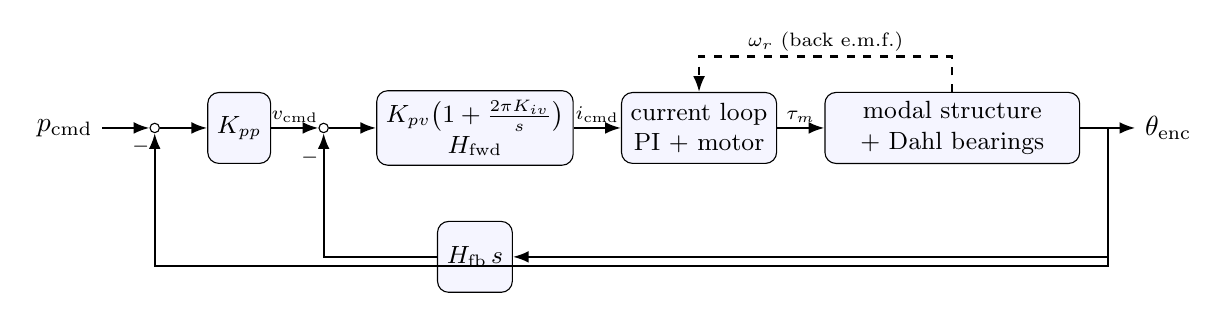
\begin{tikzpicture}[node distance=6mm]
\node (p) {$p_\mathrm{cmd}$};
\node[sum, right=of p] (s1) {};
\node[blk, right=of s1] (kp) {$K_{pp}$};
\node[sum, right=of kp] (s2) {};
\node[blk, right=of s2] (cv) {$K_{pv}\bigl(1+\frac{2\pi K_{iv}}{s}\bigr)$\\ $H_\mathrm{fwd}$};
\node[blk, right=of cv] (ci) {current loop\\ PI + motor};
\node[blk, right=of ci, text width=3.0cm] (pl) {modal structure\\ + Dahl bearings};
\node[right=7mm of pl] (y) {$\theta_\mathrm{enc}$};
\node[blk, below=7mm of cv] (hf) {$H_\mathrm{fb}\,s$};
\draw[sig] (p) -- (s1); \draw[sig] (s1) -- (kp); \draw[sig] (kp) -- node[above, lab]{$v_\mathrm{cmd}$} (s2);
\draw[sig] (s2) -- (cv); \draw[sig] (cv) -- node[above, lab]{$i_\mathrm{cmd}$} (ci);
\draw[sig] (ci) -- node[above, lab]{$\tau_m$} (pl); \draw[sig] (pl) -- (y);
\draw[sig] ($(pl.east)!0.5!(y.west)$) |- (hf.east); \draw[sig] (hf.west) -| node[pos=0.9, left, lab]{$-$} (s2.south);
\draw[sig] ($(pl.east)!0.5!(y.west)$) -- ++(0,-1.75) -| node[pos=0.95, left, lab]{$-$} (s1.south);
\draw[sig, dashed] (pl.north) -- ++(0,0.45) -| node[pos=0.25, above, lab]{$\omega_r$ (back e.m.f.)} (ci.north);
\end{tikzpicture}
\caption{Closed loop of one axis (Section~\ref{sec:cl}). In open loop (Section~\ref{sec:ol}) the measured current replaces the drive and the motor: $\tau_m=g_{K_t}K_t\,i$.}\label{fig:cl}
\end{figure}


%% ===================================================================================================
\section{Identification}\label{sec:ident}
\subsection{Computation of the error}\label{sec:cost}
This is the only change with respect to \path{report_dahl_bearings}. Each record $m$ has $N_m$ measured points $f_{m,1},\dots,f_{m,N_m}$ in the fit band. The cost is built in three steps.
\begin{enumerate}
\item \textbf{Interpolation.} The real and imaginary parts of the measured plant, and the bearing amplitude~\eqref{eq:amp}, are interpolated linearly in $f$ between the measured points:
\begin{equation}
\hat G_m(f)=\mathcal I_m[\mathrm{Re}\,G_{\mathrm{mis},m}](f)+j\,\mathcal I_m[\mathrm{Im}\,G_{\mathrm{mis},m}](f),\qquad \hat A_m(f)=\mathcal I_m[A_m](f).
\end{equation}
\item \textbf{Uniform sampling.} The interpolant is sampled on $N_m$ points between the measured extremes of the record. The number of points of the optimisation equals the number of measured points. Two grids were run:
\begin{equation}
\text{uniform in }\ln f:\ f_j=f_{m,1}\Bigl(\frac{f_{m,N_m}}{f_{m,1}}\Bigr)^{\frac{j-1}{N_m-1}},\qquad\qquad \text{uniform in }f:\ f_j=f_{m,1}+\frac{j-1}{N_m-1}\bigl(f_{m,N_m}-f_{m,1}\bigr).
\end{equation}
\item \textbf{Cost.} The error is the plain sum of the squared differences of the real and imaginary parts, with no weight:
\begin{equation}
e^2(\mathbf p)=\sum_m\sum_{j=1}^{N_m}\Bigl[\bigl(\mathrm{Re}\,G(j\omega_j;\mathbf p,\hat A_{m,j})-\mathrm{Re}\,\hat G_{m,j}\bigr)^2+\bigl(\mathrm{Im}\,G(j\omega_j;\mathbf p,\hat A_{m,j})-\mathrm{Im}\,\hat G_{m,j}\bigr)^2\Bigr].\label{eq:cost}
\end{equation}
\end{enumerate}
The parameters $\hat{\mathbf p}$ are those that minimise $e^2$. The previous report minimised $\frac12\sum_i w_i^2|G-G_\mathrm{mis}|^2$ on the measured points, with $w_i=\sqrt{\Delta\ln f_i/0.01}$. The constraints are unchanged:
\begin{itemize}
\item modal damping $\zeta_k\leq0.05$;
\item CAD inertias and stiffnesses within $\pm20$\,\%;
\item torque-constant factor $g_{K_t}\in[0.9,1.1]$ per axis (catalogue tolerance);
\item the stiffness introduced between fork base and fork top, and the stator masses (frequency and residue), free;
\item telescope rigid on the ring.
\end{itemize}
The solver is the bounded trust-region least squares of SciPy, with several starts and the covariance computed on the parameters not at a bound. All starts reach the same minimum on each axis and grid, with $e^2$ equal within about 0.02\,\%. Fit values and errors are always computed on the measured points, so all the parameter sets are comparable.

\begin{table}[H]\centering\footnotesize\setlength{\tabcolsep}{4pt}
\caption{Sampling of the records in 1--150\,Hz. $w^2$: median squared weight of the previous report. The last two columns give the points in 1--5 / 5--30 / 30--150\,Hz on each uniform grid.}\label{tab:sampling}
\begin{tabular}{lrrrrll}\toprule
record & $N_m$ & $w^2$ & step, $\ln f$ & step, $f$ & points, uniform in $\ln f$ & points, uniform in $f$ \\ \midrule
elevation, 1\,\% (1--150\,Hz) & 504 & 1.00 & 1\,\% & 0.29\,Hz & 162 / 180 / 162 & 14 / 85 / 405 \\
elevation, 1\,\% (30--150\,Hz) & 162 & 1.00 & 1\,\% & 0.74\,Hz & 0 / 0 / 162 & 0 / 0 / 162 \\
elevation, 16 screws, 2\,\% & 82 & 1.98 & 2\,\% & 1.47\,Hz & 0 / 0 / 82 & 0 / 0 / 82 \\
azimuth, 3\,\% & 170 & 2.96 & 3\,\% & 0.87\,Hz & 55 / 61 / 54 & 5 / 29 / 136
\\ \bottomrule
\end{tabular}\end{table}

\paragraph{Relation with the previous weight.} The measured grids are exact geometric grids, so the uniform $\ln f$ grid falls on the measured points (Table~\ref{tab:sampling}). Then $\hat G_{m,j}=G_{\mathrm{mis},m}(f_{m,j})$ and~\eqref{eq:cost} is the sum over the measured points with weight 1. Away from the ends of a record, the previous weight was constant within the record:
\begin{itemize}
\item \textbf{Azimuth.} There is one record, with $w^2\approx3$. The two costs differ by a constant factor and have the same minimum.
\item \textbf{Elevation.} The two 1\,\% records keep $w^2\approx1$; the 2\,\% record with 16 screws goes from $w^2\approx2$ to 1. A record now counts in proportion to its number of points.
\end{itemize}

\paragraph{Why uniform in $\ln f$ is adopted.} The uniform $f$ grid has a constant step in hertz, so the points move to high frequency (Table~\ref{tab:sampling}). Three consequences follow:
\begin{itemize}
\item the band 1--5\,Hz, where the friction acts most, keeps few points;
\item above about 30\,Hz many points fall between two measured points and are not independent data, so the standard deviations of this grid are optimistic;
\item $T_c$ of the free Dahl fit moves away from the doublet value in azimuth: \TcFreeFA\,N\,m against \TcHA\,N\,m (\TcFreeA\,N\,m with uniform $\ln f$).
\end{itemize}

\paragraph{Linear or quadratic interpolation.} On the uniform $\ln f$ grid the choice has no effect, because no point falls between two measured points. On the uniform $f$ grid a quadratic spline ($k=2$) differs from the linear interpolant by \quadSignal\,\% of the signal, or \quadResidual\,\% of the fit residual, in the order of the rows of Table~\ref{tab:sampling}. The largest differences are on the coarser grids, near the peaks. Linear interpolation is kept. The fit itself was not repeated with the quadratic interpolant.

\subsection{Hybrid identification of the bearings}
As in the previous report, the doublets determine the sliding level $T_c$ and the frequency responses the pre-sliding stiffness $\sigma_0$:
\begin{itemize}
\item the doublets move the axis by 1.7 to 280\,mrad and are almost entirely in sliding; in the time-domain identification $\sigma_0$ was fixed in the selection of the structure;
\item the frequency responses move the bearings across the pre-sliding scale.
\end{itemize}
The two domains differ on $\sigma_0$ by a factor 3 to 10 (Table~\ref{tab:friction}). With the new cost the free Dahl fit gives $T_c=\TcFreeA$\,N\,m in azimuth and \TcFreeP\,N\,m in elevation, against \TcHA\ and \TcHP\,N\,m from the doublets. The hybrid identification fixes $T_c$ at the doublet value and estimates $\sigma_0$ with the structure, with a pure Dahl element ($T_s=T_c$). Three starts were used on each axis and grid: the free Dahl fit, the previous hybrid estimate, and the latter with $\sigma_0$ from the doublets.

\begin{table}[H]\centering\footnotesize\setlength{\tabcolsep}{4pt}
\caption{Dahl parameters of the bearings. Std: relative standard deviation (``--'': not computed). Pre-sliding scale: $T_c/\sigma_0$.}\label{tab:friction}
\begin{tabular}{llrrrrr}\toprule
axis & source & $\sigma_0$ [N\,m/rad] & std & $T_c$ [N\,m] & $T_s/T_c$ & $T_c/\sigma_0$ [$\mu$rad] \\ \midrule
azimuth & doublets (V2, time domain) & 4513 & -- & 0.232 & 7.93 & 51 \\
 & hybrid, previous weights & 1571 & 1.9\,\% & 0.232 (fixed) & 1 & 147 \\
 & free Dahl, uniform in $\ln f$ & 1570 & -- & 0.204 & 1 & 130 \\
 & \textbf{hybrid, uniform in $\ln f$} & \textbf{1571} & 1.9\,\% & \textbf{0.232} (fixed) & 1 & 147 \\
 & hybrid, uniform in $f$ & 1560 & 9.2\,\% & 0.232 (fixed) & 1 & 148 \\
elevation & doublets (V2, time domain) & 1703 & -- & 0.407 & 1.14 & 239 \\
 & hybrid, previous weights & \ensuremath{1.878\times10^{4}} & 7.2\,\% & 0.407 (fixed) & 1 & 22 \\
 & free Dahl, uniform in $\ln f$ & \ensuremath{1.686\times10^{4}} & -- & 0.385 & 1 & 23 \\
 & \textbf{hybrid, uniform in $\ln f$} & \textbf{\ensuremath{1.784\times10^{4}}} & 7.4\,\% & \textbf{0.407} (fixed) & 1 & 23 \\
 & hybrid, uniform in $f$ & \ensuremath{2.027\times10^{4}} & 5.4\,\% & 0.407 (fixed) & 1 & 20
\\ \bottomrule
\end{tabular}\end{table}

%% ===================================================================================================
\section{Results: frequency domain}\label{sec:res_freq}
\subsection{Cost and fit on the Bode curves}
Three fit values are computed on the measured points, with $y$ the measured quantity:
\begin{equation}
\mathrm{fit}=100\Bigl(1-\frac{\|y_\mathrm{mod}-y\|}{\|y-\bar y\|}\Bigr)\,\%,\qquad y=G\ \text{(complex)},\quad y=20\log_{10}|G|\ \text{(magnitude)},\quad y=\angle G\ \text{(phase)}.
\end{equation}
For the phase, the differences are wrapped to $(-180^\circ,180^\circ]$ and $\bar y$ is the circular mean. The complex fit follows the cost and is dominated by the points where $|G|$ is large. The magnitude fit in dB and the phase fit also weigh the low-magnitude regions, such as the antiresonances.

\begin{table}[H]\centering\footnotesize\setlength{\tabcolsep}{4pt}
\caption{Elevation: $e^2$ of each parameter set evaluated on both uniform grids, torque factor, and rms magnitude and phase errors on the three records.}\label{tab:cost_el}
\begin{tabular}{lrrrll}\toprule
parameters from & $e^2$, grid $\ln f$ & $e^2$, grid $f$ & $g_{K_t}$ & rms [dB] & rms [deg] \\ \midrule
previous weights & \ensuremath{5.940\times10^{-4}} & \ensuremath{2.323\times10^{-4}} & 1.050 & 1.6 / 2.0 / 1.3 & 9 / 8 / 6 \\
\textbf{uniform in $\ln f$} & \ensuremath{5.909\times10^{-4}} & \ensuremath{2.241\times10^{-4}} & 1.051 & 1.6 / 2.0 / 1.4 & 9 / 8 / 7 \\
uniform in $f$ & \ensuremath{6.600\times10^{-4}} & \ensuremath{2.079\times10^{-4}} & 0.961 & 1.6 / 1.7 / 1.4 & 9 / 8 / 8
\\ \bottomrule
\end{tabular}\end{table}

\begin{table}[H]\centering\footnotesize\setlength{\tabcolsep}{4pt}
\caption{Azimuth: as Table~\ref{tab:cost_el}, one record.}\label{tab:cost_az}
\begin{tabular}{lrrrll}\toprule
parameters from & $e^2$, grid $\ln f$ & $e^2$, grid $f$ & $g_{K_t}$ & rms [dB] & rms [deg] \\ \midrule
previous weights & \ensuremath{1.782\times10^{-4}} & \ensuremath{4.885\times10^{-4}} & 0.900 & 1.6 & 15 \\
\textbf{uniform in $\ln f$} & \ensuremath{1.782\times10^{-4}} & \ensuremath{4.885\times10^{-4}} & 0.900 & 1.6 & 15 \\
uniform in $f$ & \ensuremath{2.191\times10^{-4}} & \ensuremath{4.552\times10^{-4}} & 0.900 & 1.2 & 12
\\ \bottomrule
\end{tabular}\end{table}

\begin{table}[H]\centering\scriptsize\setlength{\tabcolsep}{2.6pt}
\caption{Fit [\%] on the measured points: on the complex response, on the Bode magnitude in dB and on the phase. Whole fit band, and bands 1--5, 5--30 and 30--150\,Hz. ``--'': the record has no points in that band.}\label{tab:bode}
\begin{tabular}{llrrrrrrrrrrrr}\toprule
& & \multicolumn{4}{c}{complex} & \multicolumn{4}{c}{magnitude} & \multicolumn{4}{c}{phase} \\
\cmidrule(lr){3-6}\cmidrule(lr){7-10}\cmidrule(lr){11-14}
record & parameters from & all & 1--5 & 5--30 & 30--150 & all & 1--5 & 5--30 & 30--150 & all & 1--5 & 5--30 & 30--150 \\ \midrule
elevation, 1\,\% (1--150\,Hz) & previous weights & 78 & 82 & 35 & 73 & 78 & 81 & 42 & 63 & 84 & 71 & 49 & 91 \\
 & \textbf{uniform in $\ln f$} & 78 & 83 & 35 & 75 & 79 & 82 & 42 & 64 & 84 & 72 & 49 & 91 \\
 & uniform in $f$ & 77 & 77 & 38 & 77 & 79 & 66 & 45 & 68 & 84 & 71 & 50 & 91 \\ \addlinespace[2pt]
elevation, 1\,\% (30--150\,Hz) & previous weights & 77 & -- & -- & 77 & 63 & -- & -- & 63 & 92 & -- & -- & 92 \\
 & \textbf{uniform in $\ln f$} & 78 & -- & -- & 78 & 63 & -- & -- & 63 & 92 & -- & -- & 92 \\
 & uniform in $f$ & 79 & -- & -- & 79 & 68 & -- & -- & 68 & 91 & -- & -- & 91 \\ \addlinespace[2pt]
elevation, 16 screws, 2\,\% & previous weights & 80 & -- & -- & 80 & 75 & -- & -- & 75 & 93 & -- & -- & 93 \\
 & \textbf{uniform in $\ln f$} & 76 & -- & -- & 76 & 73 & -- & -- & 73 & 93 & -- & -- & 93 \\
 & uniform in $f$ & 75 & -- & -- & 75 & 74 & -- & -- & 74 & 91 & -- & -- & 91 \\ \addlinespace[2pt]
azimuth, 3\,\% & previous weights & 75 & 90 & 87 & 53 & 82 & 89 & 79 & 53 & 77 & 91 & 72 & 61 \\
 & \textbf{uniform in $\ln f$} & 75 & 90 & 87 & 53 & 82 & 89 & 79 & 53 & 77 & 91 & 72 & 61 \\
 & uniform in $f$ & 73 & 79 & 88 & 51 & 86 & 90 & 88 & 58 & 82 & 85 & 79 & 70
\\ \bottomrule
\end{tabular}\end{table}

\subsection{Discussion}
\paragraph{Elevation} (Tables~\ref{tab:cost_el} and \ref{tab:bode}, Figure~\ref{fig:freq_el}).
\begin{itemize}
\item \textbf{Uniform in $\ln f$.} With half the previous weight, the fit of the 16-screw record falls by 4 points and that of the 30--150\,Hz record rises by 1. The other fits change by less than 1 point. The parameters that change most are $s_{J_e}$, $s_{k_{\theta1}}$ and $s_{k_{\theta3}}$, which the data do not determine (Table~\ref{tab:hyb_el}).
\item \textbf{Uniform in $f$.} The magnitude fit in 1--5\,Hz on the main record falls from 82 to 66\,\%, while the fit of the 30--150\,Hz record improves. The factor $g_{K_t}$ falls to \gKtFP\ and $s_{J_{hp}}$ by about 7\,\%: the two compensate each other.
\item \textbf{Stator masses.} \fMassI\ and \fMassII\,Hz, with damping \zMassI\ and \zMassII\ and residues \aMassI\ and \aMassII\,(kg\,m$^2$)$^{-1}$.
\end{itemize}

\paragraph{Azimuth} (Tables~\ref{tab:cost_az} and \ref{tab:bode}, Figure~\ref{fig:freq_az}).
\begin{itemize}
\item \textbf{Uniform in $\ln f$.} The estimate is identical to the previous one. The fork mode keeps $\zeta=\zForkA$, $\alpha=\alphaA$ and $k_{LA}=$\,\kLA\,N\,m/rad. The torque factor stays at its lower bound, $g_{K_t}=\gKtA$.
\item \textbf{Uniform in $f$.} The complex fit falls from 75 to 73\,\% and in 1--5\,Hz from 90 to 79\,\%. The magnitude fit rises from 82 to 86\,\% and the phase fit from 77 to 82\,\%, with an rms error of 1.2\,dB against 1.6\,dB. The antiresonance near 12\,Hz is closer to the measured one. On this axis the Bode curves favour the uniform $f$ grid above 5\,Hz, while the phase in 1--5\,Hz is worse. The stiffness $k_{LA}$ falls by about 15\,\% and $\zeta$ of the fork mode rises by about 43\,\%.
\end{itemize}

\paragraph{Other bearing models.} The linear hysteretic, LuGre and time-domain Dahl models compared in \path{report_dahl_bearings} were not identified again with the new cost. The choice of the hybrid Dahl element rests on that report. For the azimuth, where the two costs have the same minimum, its comparison holds unchanged.

\begin{figure}[H]\centering
\includegraphics[width=0.94\linewidth]{figures/freq_elevation.pdf}
\caption{Elevation plant [dB (rad/s)/A] and phase: measurements and hybrid models from the three costs. Legend: complex fit on the three records.}\label{fig:freq_el}
\end{figure}

\begin{figure}[H]\centering
\includegraphics[width=0.94\linewidth]{figures/freq_azimuth.pdf}
\caption{Azimuth plant and phase: as Figure~\ref{fig:freq_el}, one record.}\label{fig:freq_az}
\end{figure}

\begin{figure}[H]\centering
\includegraphics[width=0.95\linewidth]{figures/df_resampled.pdf}
\caption{Describing function of the bearings at the measured amplitude (first record of each axis) for the three hybrid parameter sets: magnitude, loss factor, and bearing amplitude~\eqref{eq:amp} against the pre-sliding scale $T_c/\sigma_0$ (horizontal lines).}\label{fig:df_amp}
\end{figure}

\begin{table}[H]\centering\scriptsize\setlength{\tabcolsep}{3pt}
\caption{Hybrid model, elevation: parameters from the three costs. Std and ``at bound'' refer to the adopted estimate (uniform in $\ln f$).}\label{tab:hyb_el}
\begin{tabular}{lL{2.4cm}lrrrlrl}\toprule
param. & class & unit & previous & \textbf{uniform $\ln f$} & uniform $f$ & bounds & std & at bound \\ \midrule
$s_{J_e}$ & CAD, $\pm20$\,\% & -- & 0.8585 & \textbf{1.157} & 0.8968 & [0.8, 1.2] & n.d. &  \\
$s_{J_{hp}}$ & CAD, $\pm20$\,\% & -- & 0.9979 & \textbf{1.001} & 0.9275 & [0.8, 1.2] & 1.3\,\% &  \\
$s_{J_m}$ & CAD, $\pm20$\,\% & -- & 0.8 & \textbf{0.8} & 0.8 & [0.8, 1.2] & -- & yes \\
$s_{J_\mathrm{rear}}$ & CAD, $\pm20$\,\% & -- & 0.8 & \textbf{0.8} & 0.8 & [0.8, 1.2] & -- & yes \\
$s_{k_{\theta1}}$ & CAD, $\pm20$\,\% & -- & 0.9155 & \textbf{1.052} & 1.19 & [0.8, 1.2] & n.d. &  \\
$s_{k_{\theta2}}$ & CAD, $\pm20$\,\% & -- & 1.2 & \textbf{1.2} & 1.2 & [0.8, 1.2] & -- & yes \\
$s_{k_{\theta3}}$ & CAD, $\pm20$\,\% & -- & 0.9138 & \textbf{1.18} & 1.149 & [0.8, 1.2] & n.d. &  \\
$\sigma_0$ & bearings, free & N\,m/rad & \ensuremath{1.878\times10^{4}} & \textbf{\ensuremath{1.784\times10^{4}}} & \ensuremath{2.027\times10^{4}} & [10, \ensuremath{1\times10^{7}}] & 7.4\,\% &  \\
$T_c$ & bearings, doublets & N\,m & 0.4073 & 0.4073 & 0.4073 & fixed & -- &  \\
$\tau_d$ & drive & s & 0.0004709 & \textbf{0.0004685} & 0.0005716 & [\ensuremath{1\times10^{-6}}, 0.002] & 10.3\,\% &  \\
$f_1$ & stator mass, free & Hz & 56 & \textbf{56.13} & 56.17 & [40, 80] & 0.1\,\% &  \\
$a_1$ & stator mass, free & (kg\,m$^2$)$^{-1}$ & $-$0.5549 & \textbf{$-$0.5484} & $-$0.6167 & [$-$50, 50] & 3.2\,\% &  \\
$f_2$ & stator mass, free & Hz & 98.24 & \textbf{98.29} & 98.29 & [80, 140] & 0.2\,\% &  \\
$a_2$ & stator mass, free & (kg\,m$^2$)$^{-1}$ & 0.6066 & \textbf{0.5909} & 0.6019 & [$-$50, 50] & 4.8\,\% &  \\
$g_{K_t}$ & motor, $\pm10$\,\% & -- & 1.05 & \textbf{1.051} & 0.9608 & [0.9, 1.1] & 0.7\,\% &  \\
$\zeta_2$ & modal, $\leq0.05$ & -- & 0.01922 & \textbf{0.02065} & 0.01996 & [0.0001, 0.05] & 6.4\,\% &  \\
$\zeta_3$ & modal, $\leq0.05$ & -- & 0.0309 & \textbf{0.03036} & 0.02795 & [0.0001, 0.05] & 6.9\,\% &  \\
$\zeta_4$ & modal, $\leq0.05$ & -- & 0.0001 & \textbf{0.0001} & 0.0001 & [0.0001, 0.05] & -- & yes \\
$\zeta_5$ & modal, $\leq0.05$ & -- & 0.0001 & \textbf{0.0001} & 0.0001 & [0.0001, 0.05] & -- & yes \\
$\zeta_6$ & modal, $\leq0.05$ & -- & 0.0001969 & \textbf{0.0001017} & 0.0001 & [0.0001, 0.05] & n.d. & 
\\ \bottomrule
\end{tabular}\end{table}

\begin{table}[H]\centering\scriptsize\setlength{\tabcolsep}{3pt}
\caption{Hybrid model, azimuth: as Table~\ref{tab:hyb_el}.}\label{tab:hyb_az}
\begin{tabular}{lL{2.4cm}lrrrlrl}\toprule
param. & class & unit & previous & \textbf{uniform $\ln f$} & uniform $f$ & bounds & std & at bound \\ \midrule
$s_{J_e}$ & CAD, $\pm20$\,\% & -- & 0.8 & \textbf{0.8} & 0.8 & [0.8, 1.2] & -- & yes \\
$s_{J_m}$ & CAD, $\pm20$\,\% & -- & 0.8 & \textbf{0.8} & 0.8 & [0.8, 1.2] & -- & yes \\
$s_{J_L}$ & CAD, $\pm20$\,\% & -- & 1.135 & \textbf{1.135} & 1.046 & [0.8, 1.2] & 1.2\,\% &  \\
$s_{k_1}$ & CAD, $\pm20$\,\% & -- & 1.2 & \textbf{1.2} & 1.2 & [0.8, 1.2] & -- & yes \\
$s_{k_2}$ & CAD, $\pm20$\,\% & -- & 1.2 & \textbf{1.2} & 1.2 & [0.8, 1.2] & -- & yes \\
$\alpha$ & introduced, free & -- & 0.6066 & \textbf{0.6066} & 0.6441 & [0.02, 0.98] & 2.1\,\% &  \\
$k_{LA}$ & introduced, free & N\,m/rad & \ensuremath{5.474\times10^{4}} & \textbf{\ensuremath{5.474\times10^{4}}} & \ensuremath{4.672\times10^{4}} & [\ensuremath{1\times10^{3}}, \ensuremath{1\times10^{8}}] & 2.3\,\% &  \\
$\sigma_0$ & bearings, free & N\,m/rad & 1571 & \textbf{1571} & 1560 & [10, \ensuremath{1\times10^{7}}] & 1.9\,\% &  \\
$T_c$ & bearings, doublets & N\,m & 0.2316 & 0.2316 & 0.2316 & fixed & -- &  \\
$\tau_d$ & drive & s & 0.0004781 & \textbf{0.0004781} & 0.0004472 & [\ensuremath{1\times10^{-6}}, 0.002] & 4.2\,\% &  \\
$g_{K_t}$ & motor, $\pm10$\,\% & -- & 0.9 & \textbf{0.9} & 0.9 & [0.9, 1.1] & -- & yes \\
$\zeta_2$ & modal, $\leq0.05$ & -- & 0.02818 & \textbf{0.02818} & 0.04029 & [0.0001, 0.05] & 6.0\,\% &  \\
$\zeta_3$ & modal, $\leq0.05$ & -- & 0.0001 & \textbf{0.0001} & 0.0001 & [0.0001, 0.05] & -- & yes \\
$\zeta_4$ & modal, $\leq0.05$ & -- & 0.05 & \textbf{0.05} & 0.05 & [0.0001, 0.05] & -- & yes
\\ \bottomrule
\end{tabular}\end{table}

%% ===================================================================================================
\section{Results: doublets, summary}\label{sec:res_sum}
Table~\ref{tab:med} summarises the two verifications of Sections~\ref{sec:res_ol} and~\ref{sec:res_cl}. No plant parameter is estimated on these data.
\begin{table}[H]\centering\footnotesize
\caption{Median fit [\%] during the moves, over the 18 moves of each axis (17 in azimuth: the first move of the 8$^\circ$ doublet is excluded, see Section~\ref{sec:res_cl}).}\label{tab:med}
\begin{tabular}{llrrr}\toprule
axis & parameters from & open loop, position & closed loop, position & closed loop, current \\ \midrule
azimuth & previous weights & 42.4 & 96.0 & 20.1 \\
 & \textbf{uniform in $\ln f$} & 42.4 & 96.0 & 20.1 \\
 & uniform in $f$ & 53.1 & 95.8 & 25.6 \\
elevation & previous weights & 13.3 & 95.7 & 50.1 \\
 & \textbf{uniform in $\ln f$} & 13.3 & 95.7 & 50.0 \\
 & uniform in $f$ & $-$3.2 & 95.7 & 46.4
\\ \bottomrule
\end{tabular}\end{table}

%% ===================================================================================================
\section{Results: doublets in open loop (measured current in)}\label{sec:res_ol}
The hybrid model is driven by the measured current. Table~\ref{tab:ol} gives the position fit during each move, from the start of the reference to 0.5\,s after its end.

\begin{table}[H]\centering\footnotesize\setlength{\tabcolsep}{4pt}
\caption{Open loop: NRMSE fit [\%] of the encoder position during the three moves of each doublet, for the two uniform grids.}\label{tab:ol}
\begin{tabular}{lllll}\toprule
& \multicolumn{2}{c}{azimuth} & \multicolumn{2}{c}{elevation} \\
\cmidrule(lr){2-3}\cmidrule(lr){4-5}
amplitude [$^\circ$] & uniform $\ln f$ & uniform $f$ & uniform $\ln f$ & uniform $f$ \\ \midrule
0.1 & $-$1532 / $-$13 / $-$149 & $-$1689 / $-$8 / $-$184 & 38 / $-$63 / $-$54 & $-$9 / $-$71 / $-$56 \\
0.5 & 33 / 44 / 86 & 13 / 56 / 84 & 21 / 9 / 23 & 90 / $-$5 / $-$2 \\
1 & 64 / 49 / 59 & 77 / 61 / 72 & 43 / $-$54 / 58 & 92 / $-$15 / 41 \\
3 & 82 / 42 / 31 & 90 / 53 / 41 & 4 / $-$34 / 58 & 70 / $-$29 / 43 \\
5 & 75 / 54 / 27 & 59 / 65 / 37 & 37 / $-$34 / 37 & 69 / $-$42 / 23 \\
8 & $-$40 / 23 / 23 & $-$29 / 32 / 32 & 17 / $-$83 / 6 & 52 / $-$81 / $-$12
\\ \bottomrule
\end{tabular}\end{table}

\begin{itemize}
\item \textbf{Start of the moves.} The acceleration, the oscillation of about 7\,Hz imposed by the controller and the braking are reproduced at the start of the moves (Figures~\ref{fig:ol_az}, \ref{fig:ol_el}).
\item \textbf{Drift at rest.} At rest the real axis holds torques above $T_c$. A pure Dahl element cannot exceed $T_c$, so the model slides and drifts, with all three parameter sets. In elevation the drift starts later with the uniform $f$ set.
\item \textbf{Torque in azimuth.} The model is short of torque: peak velocity about 0.065 against 0.080\,rad/s at 1$^\circ$, cruise velocity about 0.125 against 0.175\,rad/s at 5$^\circ$ with uniform $\ln f$. The uniform $f$ set is slightly closer. The result depends on the scale of the current channel (Section~\ref{sec:limits}).
\item \textbf{Why open loop is ill conditioned.} A current-driven axis integrates any torque error twice. The open-loop test is therefore sensitive to the holding torques and to the current scale, not only to the plant. The differences between the grids in Table~\ref{tab:med} should be read with this in mind.
\end{itemize}

\begin{figure}[H]\centering
\includegraphics[width=\linewidth]{figures/ol_azimuth.pdf}
\caption{Azimuth, open loop: encoder position, velocity and input current for one move of the 0.1, 1 and 5$^\circ$ doublets; measurement and hybrid models from the three costs.}\label{fig:ol_az}
\end{figure}

\begin{figure}[H]\centering
\includegraphics[width=\linewidth]{figures/ol_elevation.pdf}
\caption{Elevation, open loop: as Figure~\ref{fig:ol_az}.}\label{fig:ol_el}
\end{figure}

%% ===================================================================================================
\section{Results: doublets in closed loop (position reference in)}\label{sec:res_cl}
\paragraph{Gains of the drives.} With the gains of the \texttt{.akd} files and of the WorkBench exports, the previous report found that the model does not reproduce the doublets: in azimuth, largest following error \akdErrA\,mdeg against \akdErrMeasA\,mdeg measured and current command up to \akdImaxA\,A against \akdImaxMeasA\,A; in elevation, \akdErrP\,mdeg against \akdErrMeasP\,mdeg. That run was not repeated. The effective gains $K_{pp}$, $K_{pv}$, $K_{iv}$ are estimated for each parameter set with the same procedure:
\begin{itemize}
\item on the following error of the 1$^\circ$ doublet only, with the plant fixed;
\item starting from the values of \path{closedLoopModel}.
\end{itemize}
The current is not used in the estimate. The gains absorb part of the differences between the parameter sets: $K_{pv}$ in azimuth is 8.5\,\% lower with the uniform $f$ set (Table~\ref{tab:gains}).

\begin{table}[H]\centering\footnotesize\setlength{\tabcolsep}{4pt}
\caption{Gains of the position and velocity loops. $K_{pp}$ [1/s], $K_{pv}$ [A/(rad/s)], $K_{iv}$ [Hz].}\label{tab:gains}
\begin{tabular}{llrrr}\toprule
axis & source & $K_{pp}$ & $K_{pv}$ & $K_{iv}$ \\ \midrule
azimuth & files (.akd, WorkBench) & 62.83 & 250 & 1.00 \\
 & \texttt{closedLoopModel} (September) & 7.43 & 198 & 0.15 \\
 & V2, 1$^\circ$, previous weights & 7.92 & 187 & 0.37 \\
 & V2, 1$^\circ$, \textbf{uniform in $\ln f$} & 7.92 & 187 & 0.37 \\
 & V2, 1$^\circ$, uniform in $f$ & 7.95 & 171 & 0.39 \\
elevation & files (.akd, WorkBench) & 2.51 & 25 & 15.00 \\
 & \texttt{closedLoopModel} (September) & 8.58 & 61 & 0.73 \\
 & V2, 1$^\circ$, previous weights & 8.02 & 53 & 1.28 \\
 & V2, 1$^\circ$, \textbf{uniform in $\ln f$} & 8.02 & 54 & 1.28 \\
 & V2, 1$^\circ$, uniform in $f$ & 8.15 & 55 & 1.24
\\ \bottomrule
\end{tabular}\end{table}

\begin{table}[H]\centering\scriptsize\setlength{\tabcolsep}{3pt}
\caption{Closed loop, adopted estimate (uniform in $\ln f$): NRMSE fit [\%] of the encoder position over the window and during the move (to 1\,s after the end of the reference), and of the current during the move, for the three moves of each doublet. Estimation set: the 1$^\circ$ doublet (gains only).}\label{tab:cl}
\begin{tabular}{lllllll}\toprule
& \multicolumn{3}{c}{azimuth} & \multicolumn{3}{c}{elevation} \\
\cmidrule(lr){2-4}\cmidrule(lr){5-7}
ampl. [$^\circ$] & pos., window & pos., move & current & pos., window & pos., move & current \\ \midrule
0.1 & 91 / 83 / 89 & 86 / 61 / 73 & 14 / $-$13 / 10 & 55 / 71 / 52 & $-$5 / 31 / $-$20 & 12 / 51 / 24 \\
0.5 & 96 / 98 / 96 & 91 / 95 / 91 & 13 / 17 / 15 & 95 / 98 / 97 & 91 / 97 / 94 & 36 / 50 / 19 \\
1 & 98 / 99 / 98 & 96 / 97 / 95 & 15 / 36 / 16 & 98 / 98 / 98 & 96 / 97 / 96 & 21 / 60 / 54 \\
3 & 98 / 99 / 99 & 96 / 98 / 97 & 28 / 26 / 24 & 96 / 98 / 97 & 92 / 97 / 95 & 51 / 55 / 63 \\
5 & 98 / 99 / 99 & 97 / 99 / 98 & 37 / 24 / 25 & 97 / 99 / 98 & 95 / 98 / 96 & 50 / 45 / 60 \\
8 & $-$136 / 100 / 99 & $-$92 / 99 / 98 & $-$56 / 20 / 26 & 98 / 99 / 99 & 97 / 99 / 97 & 35 / 27 / 56
\\ \bottomrule
\end{tabular}\end{table}

\begin{table}[H]\centering\scriptsize\setlength{\tabcolsep}{3.5pt}
\caption{Closed loop: largest following error [mdeg] and largest current [A$_\mathrm{rms}$] during the moves, median of the three moves; measurement and models from the two uniform grids.}\label{tab:cl_peaks}
\begin{tabular}{lrrrrrrrrrrrr}\toprule
& \multicolumn{6}{c}{azimuth} & \multicolumn{6}{c}{elevation} \\
\cmidrule(lr){2-7}\cmidrule(lr){8-13}
& \multicolumn{3}{c}{error [mdeg]} & \multicolumn{3}{c}{current [A]} & \multicolumn{3}{c}{error [mdeg]} & \multicolumn{3}{c}{current [A]} \\
\cmidrule(lr){2-4}\cmidrule(lr){5-7}\cmidrule(lr){8-10}\cmidrule(lr){11-13}
ampl. [$^\circ$] & meas. & $\ln f$ & $f$ & meas. & $\ln f$ & $f$ & meas. & $\ln f$ & $f$ & meas. & $\ln f$ & $f$ \\ \midrule
0.1 & 96 & 95 & 95 & 4.6 & 3.5 & 3.3 & 100 & 99 & 100 & 1.8 & 1.6 & 1.8 \\
0.5 & 410 & 421 & 422 & 9.3 & 7.9 & 7.3 & 450 & 439 & 441 & 4.0 & 3.6 & 3.8 \\
1 & 721 & 757 & 758 & 10.2 & 11.0 & 10.2 & 837 & 822 & 821 & 5.8 & 4.9 & 5.1 \\
3 & 1295 & 1283 & 1282 & 10.3 & 11.6 & 10.8 & 1298 & 1283 & 1274 & 5.7 & 5.8 & 6.1 \\
5 & 1296 & 1282 & 1281 & 10.3 & 11.6 & 10.8 & 1314 & 1297 & 1292 & 5.8 & 5.9 & 6.1 \\
8 & 1296 & 1283 & 1282 & 9.9 & 11.6 & 10.8 & 1310 & 1297 & 1295 & 5.7 & 5.9 & 6.1
\\ \bottomrule
\end{tabular}\end{table}

\paragraph{What agrees} (Tables~\ref{tab:cl}, \ref{tab:cl_peaks}; Figures~\ref{fig:cl_az}, \ref{fig:cl_el}).
\begin{itemize}
\item \textbf{Position and following error.} From 0.5 to 8$^\circ$ the position fit over the window is \clFitMinA--\clFitMaxA\,\% in azimuth and \clFitMinP--\clFitMaxP\,\% in elevation. The exception is the first move of the 8$^\circ$ azimuth doublet, whose window is cut by the detection of the moves. The model reproduces acceleration, the cruise at 10$^\circ$/s with about 1.3$^\circ$ of following error, braking and settling.
\item \textbf{Current peaks.} From 1 to 8$^\circ$, the ratio of the largest model current to the measured one has median \iRatioMedA\ in azimuth (range \iRatioMinA--\iRatioMaxA) and \iRatioMedP\ in elevation (range \iRatioMinP--\iRatioMaxP), with the current scale \texttt{AMPS}~$=2I_\mathrm{rms}$. The largest current command in the simulations is \icmdMaxA\,A in azimuth and \icmdMaxP\,A in elevation, below the drive limit of 18\,A.
\end{itemize}

\paragraph{What differs.} These differences are common to the three parameter sets.
\begin{itemize}
\item \textbf{Azimuth current near 7\,Hz.} After the first peak the measured current oscillates for 3--4 periods with amplitude up to $\pm10$\,A, while the model is damped; the effect on the position is small. The current fit during the moves stays low (Table~\ref{tab:med}). It is a dynamics of the friction or of the real loop that the pure Dahl element does not give.
\item \textbf{Small moves and rest in elevation.} At 0.1$^\circ$ the model sticks about 0.25\,s longer than the real axis before moving. After the moves the real axis stops a few millidegrees short, then creeps to the reference while the current grows; the model reaches the reference earlier and holds less current. This is stick-slip behaviour, with a static torque above $T_c$, that a pure Dahl element does not represent.
\end{itemize}

\begin{figure}[H]\centering
\includegraphics[width=\linewidth]{figures/cl_azimuth.pdf}
\caption{Azimuth, closed loop with the measured position reference: position, following error and motor current for one move of the 0.1, 1 and 5$^\circ$ doublets; measurement and models from the three costs (AKD2G drive with the effective gains of each set, TBM7646 motor, hybrid Dahl plant).}\label{fig:cl_az}
\end{figure}

\begin{figure}[H]\centering
\includegraphics[width=\linewidth]{figures/cl_elevation.pdf}
\caption{Elevation, closed loop: as Figure~\ref{fig:cl_az}.}\label{fig:cl_el}
\end{figure}

%% ===================================================================================================
\section{Limitations and open points}\label{sec:limits}
\begin{itemize}
\item \textbf{Overlapping records.} The cost is summed per record, so the band 30--150\,Hz, covered by three elevation records, holds \overlapShare\,\% of the elevation points (59\,\% of the sum of $w^2$ in the previous report). Removing the weight does not remove this. Each record still counts in proportion to its number of points.
\item \textbf{Independence of the points.} On the uniform $f$ grid the interpolated points are not independent measurements, so the standard deviations of that grid are optimistic. On the uniform $\ln f$ grid every point is a measured point.
\item \textbf{Comparison with other bearing models.} Linear hysteretic, LuGre and time-domain Dahl bearings were not identified again with the new cost, and the standard deviations of the free Dahl fit were not computed.
\item \textbf{Amplitude of the bearings in frequency.} The bearing amplitude~\eqref{eq:amp} is taken from the measured response, so the describing function partly inherits the measured shape. The predictive version is the self-consistent harmonic balance in closed loop described in \path{report_dahl_bearings}. It is not implemented yet.
\item \textbf{Scale of the current channel.} \texttt{AXIS*\_AMPS} is taken as $2I_\mathrm{rms}$, as in \path{closedLoopModel}. The arguments for and against are in \path{report_dahl_bearings}. It can be settled from the definition of the channel in the PLC program, or by recording \texttt{IL.FB} with the WorkBench scope together with the PLC channel.
\item \textbf{Effective loop of the PLC.} The gains of the drive files do not reproduce the doublets; three effective gains per axis are estimated from them. They should be checked against the actual configuration of the PLC (MPCLucy).
\item \textbf{Static friction and holding torques.} The pure Dahl element holds at most $T_c$. The measured holding torques at rest and the creep after the moves require a static torque above $T_c$, or position-dependent torques (cables, unbalance).
\item \textbf{Torque constant in azimuth.} $g_{K_t}$ stays at its lower bound (0.90) with every cost. Together with the scale of the current channel, this is the open point on the ratio $K_t/J$ of the azimuth axis.
\end{itemize}

\paragraph{Reproducibility.} From \path{sim/gimbal_multidof}:
\begin{itemize}
\item \texttt{analisi\_dahl\_ricampionato.py}: identification on the two uniform grids, interpolation comparison;
\item \texttt{analisi\_fit\_bode\_ricampionato.py}: fit on the Bode curves, sampling, frequency-domain figures;
\item \texttt{analisi\_tempo\_ricampionato.py}: open loop, closed loop, effective gains;
\item \texttt{report\_dahl\_resampled/build\_dahl\_resampled\_report.py}: this report.
\end{itemize}
The results are in \path{results_fork_modes_dahl_resampled}. The model code is in \path{src/gimbal_mdof/forcella_lugre.py} (describing function, plant) and \path{src/gimbal_mdof/doppietti_tempo.py} (time-domain simulation).

\end{document}
